\chapter{\label{ch:wavelets}Wavelets}
In previous chapter, chapter \ref{ch:projection}, we discussed numerical solution of radiosity integral equation using projection method. Basically we select space and basis for that space for projection. In this chapter we discuss wavelet basis, which are hierarchical basis which can be used as an alternative basis for well known finite dimensional spaces, associated properties like vanishing moments. Good text on wavelet can be found in \cite{book:goswami} \cite{book:Stollnitz}. In next chapter, chapter \ref{ch:waveletprojection}, we discuss the advantage of wavelet basis over other basis and comparison of different wavelets for solving problem. First the basics of wavelet and Haar wavelet is discussed. Then a class of wavelet called multi-wavelets and Legendre multi-wavelets is discussed.\\
% \section{Wavelet}
% Wavelet constitute a family of functions constructed from dilation and translation of a single function called the mother wavelet. When the dilation parameter a and the translation parameter b vary continuously, we have the following family of continuous wavelets \cite{book:boggess} as 
% \begin{equation}
% \psi_{a,b}(x) = {|a|}^{-1} \psi(\frac {t-b}{a}),\quad a,b \in R, a \neq 0
% \end{equation}
% If we restrict the parameters $a$ and $b$ to the discrete values as $a = a_0 ^-k, \\b = n b_0 a_0^{-k}$, where $a>1,b>0$ and $n =..., -2, -1, 0, 1, 2,...,k=0,1,2,...$, we have the following of discrete wavelets:\\
% \begin{equation}\label{eq:discreate}
% \psi_{n,k}(x) = |a|^\frac{k}{2} \psi(a_0^k t - nb_0) ,\\
% \end{equation}
%  which from a wavelet basis for $L^2(R)$. In particular, when $a_0 = 2$ and $b_0 = 1$ then $\psi_{n,k} (x)$ forms an orthonormal dyadic wavelet basis \cite{book:goswami}. Haar wavelet being simplest wavelet is first described and  then Legendre wavelets has been described in next sections.


\section{Haar Wavelet}
Haar wavelet is simplest wavelet, which can be explained easily. Haar wavelet consist of single mother wavelet $\psi_0(x)$(see Figure \ref{fig:haarpsi}), single scaling function $\phi_0(x)$(see Figure \ref{fig:haarphi}), and dilates/translates of mother wavelet as shown in Equation \ref{eq:discreate}.  Thus orthonormal Haar wavelet basis for $L^2$ space is list of functions shown below

\begin{equation}\label{eq:haarbasis}
(\phi_0(x),\psi_{n,k}(x)),\quad  n= 1, 2,...\quad  \text{and} \quad k=0,1,2,...,2^n-1
\end{equation}
If we select finite subset of the set in Equation \ref{eq:haarbasis}, we can form basis for space of piece-vice constant functions as discussed in Chapter \ref{ch:projection}. For example for function space discussed in Chapter \ref{ch:projection}, we have $m=1$ and $n=4$ to get space of piece-vice constant function over standard interval of size $\frac{1}{4}$. Thus we have 4 intervals and we need 4 basis function to span this space. Haar basis for this space is shown below
\begin{equation}\label{eq:haarbasis_n4}
(\phi_0(x),\psi_0(x),\psi_{n,k}(x)),\quad n= 1 \quad \text{and} \quad k=0,1,2,...,2^n-1
\end{equation}
where, $\psi_{n,k}(x)=\psi_{0}(2^n x+k)$.
Use of Haar wavelet as basis for space for approximating radiosity function is described in Chapter \ref{ch:waveletprojection}.



\begin{figure*}
\centering
\subfloat[Mother Wavelet Function: $\phi(x)$]{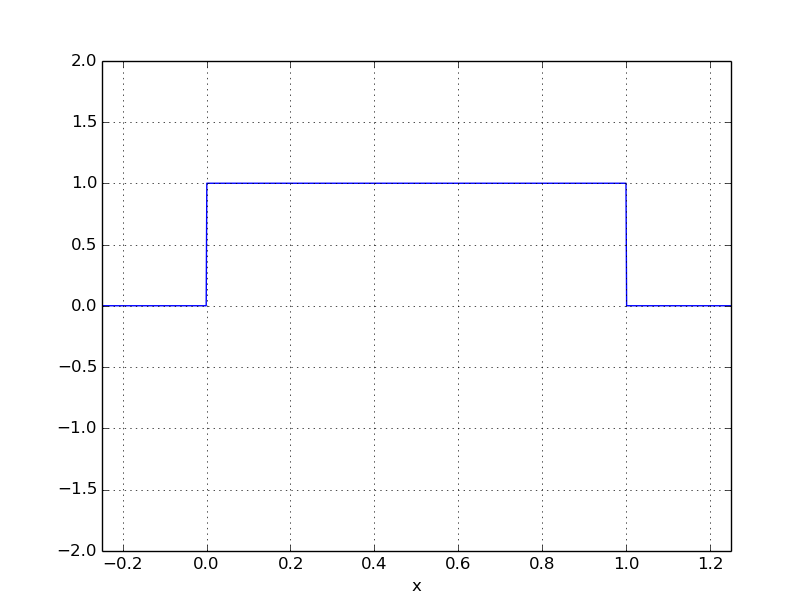
\includegraphics[width=3in]{haarphi.png}
\label{fig:haarphi}
}
\subfloat[Scaling Function: $\psi(x)$]{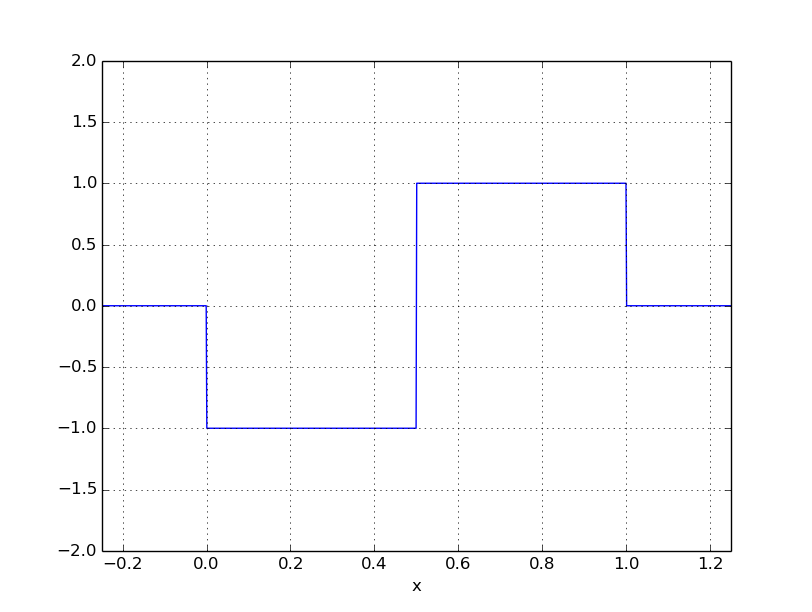
\includegraphics[width=3in]{haarpsi.png}
\label{fig:haarpsi}
}\\
\caption{Haar Wavelet}
\label{fig:haarphipsi}
\end{figure*}


 

 \section{Legendre Multi-wavelets}
Multi-wavelets are wavelets which have multiple mother wavelet  functions and scaling functions $\psi^i(x), \phi^i(x),\quad i=0,1,2,...$. They are not true wavelet as it dose not have single mother wavelet. Legendre multi-wavelet is one of the multi-wavelet. Linear Legendre multi-wavelet have two mother wavelet functions $\psi^0(x), \psi^1(x)$ and two scaling functions $\phi^0(x), \phi^1(x)$ (see Figure \ref{fig:llmwphipsi}). 

\begin{equation}
\phi^0(x)=
\left\{
    \begin{array}{ll}
        1  & \mbox{if } 0 \leq x < 1 \\
        0 & elsewhere
    \end{array}
\right.
\end{equation}
\begin{equation}
\phi^1(x)=
\left\{
    \begin{array}{ll}
        \sqrt{3}(2x-1)  & \mbox{if } 0 \leq x < 1 \\
        0 & elsewhere
    \end{array}
\right.
\end{equation}

\begin{equation}
\psi^0(x)=
\left\{
    \begin{array}{ll}
        -\sqrt{3}(4x-1)  & \mbox{if } 0 \leq x < \frac{1}{2} \\
        \sqrt{3}(4x-1)  & \mbox{if } \frac{1}{2} \leq x < 1 \\
        0 & elsewhere
    \end{array}
\right.
\end{equation}

\begin{equation}
\psi^1(x)=
\left\{
    \begin{array}{ll}
        (6x-1)  & \mbox{if } 0 \leq x < \frac{1}{2} \\
        (6x-5)  & \mbox{if } \frac{1}{2} \leq x < 1 \\
        0 & elsewhere
    \end{array}
\right.
\end{equation}

\begin{figure*}
\centering
\subfloat[Scaling Function:  $\phi^0(x)$]{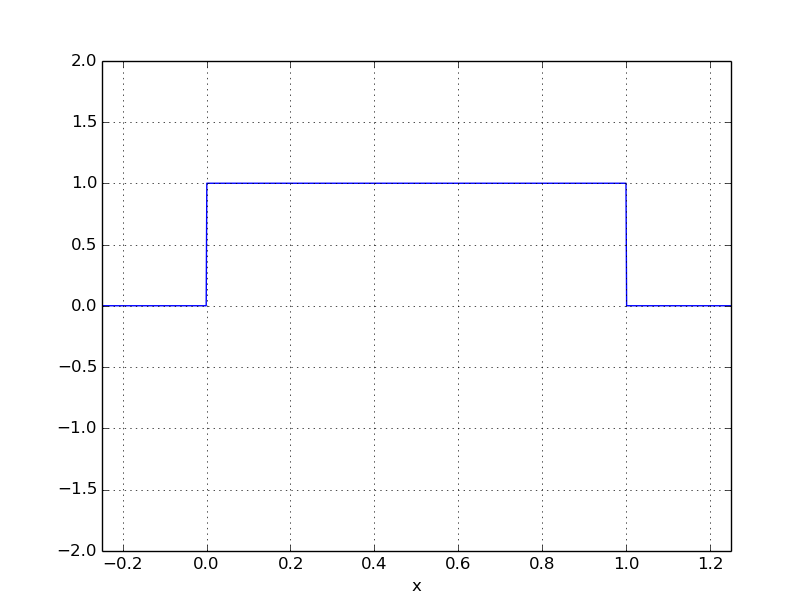
\includegraphics[width=3in]{llmwphi0.png}
\label{fig:llmwphi0}
}\subfloat[Scaling Function:  $\phi^1(x)$]{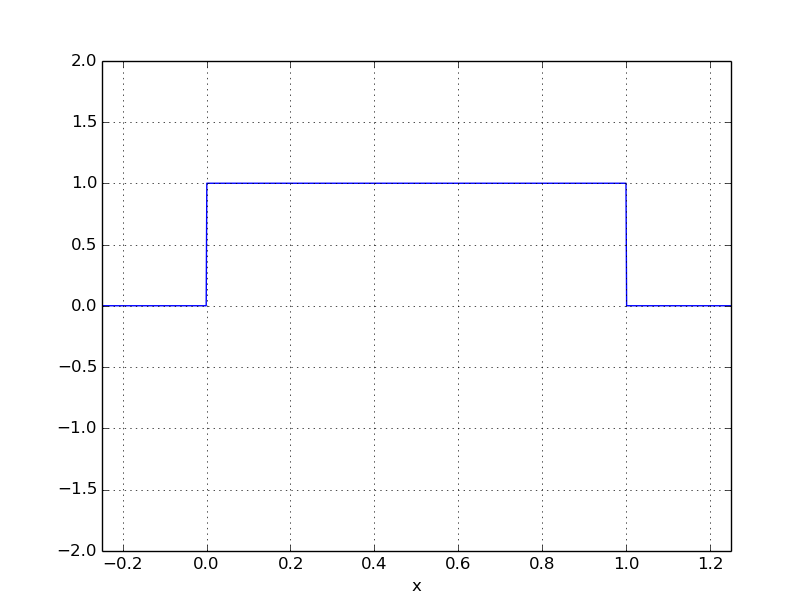
\includegraphics[width=3in]{llmwphi1.png}
\label{fig:llmwphi1}
}\\
\subfloat[Mother Wavelet Function:  $\psi^0(x)$]{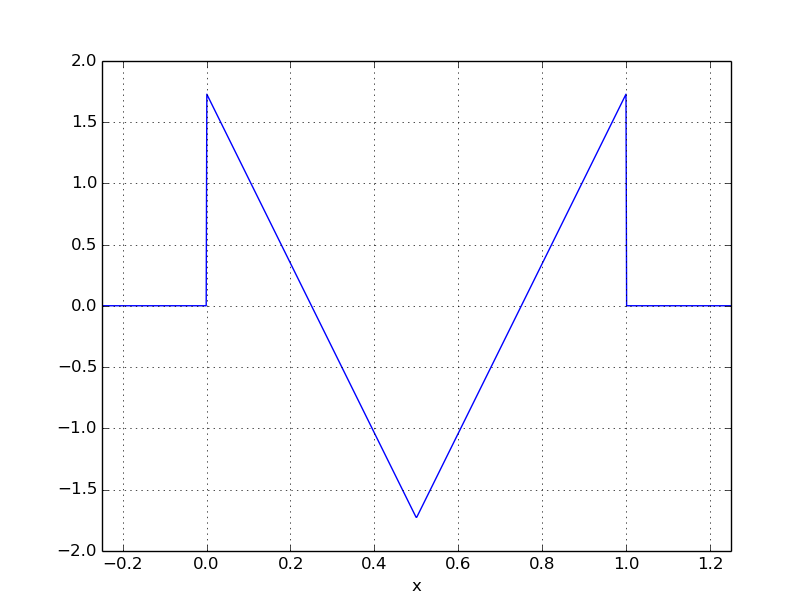
\includegraphics[width=3in]{llmwpsi0.png}
\label{fig:llmwpsi0}
}\subfloat[Mother Wavelet Function:  $\psi^1(x)$]{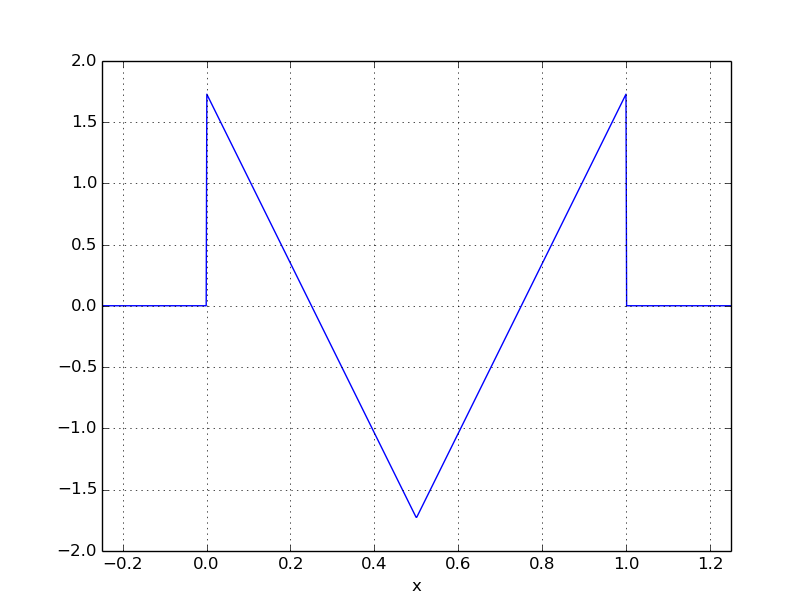
\includegraphics[width=3in]{llmwpsi1.png}
\label{fig:llmwpsi1}
}\\
\caption{Linear Legendre Multi-wavelet}
\label{fig:llmwphipsi}
\end{figure*}
% The two scale relationship of LLMW is $4 \times 4$~matrix
% \begin{equation}
% \left[ \begin{array}{c} x_1 \\ x_2 \end{array} \right] = \begin{bmatrix} A & B \\ C & D \end{bmatrix} \times \left[ \begin{array}{c} y_1 \\ y_2 \end{array} \right]
% \end{equation}
% \underline{Find way to show this thing}
% \[ \left( \begin{array}{ccc}
% % a & b & \frac{1}{\sqrt{2}} \\
% % d & e & f \\
% % g & h & i
% \frac{1}{\sqrt{2}}   &   a   &   \frac{1}{\sqrt{2}}   &   b \\

% -\frac{\sqrt{3}}{\sqrt{8}}  & \frac{1}{\sqrt{2}} & \frac{\sqrt{3}}{\sqrt{8}} & \frac{1}{\sqrt{2}} \\
% b  & \frac{1}{\sqrt{2}} & b & \frac{1}{\sqrt{2}} \\
% \frac{1}{\sqrt{2}}  & -\frac{\sqrt{3}}{\sqrt{8}} & -\frac{1}{\sqrt{2}} & -\frac{\sqrt{3}}{\sqrt{8}} 
%  \end{array} \right)\] 
Thus LLMW basis for $L^2$ space is list of functions shown below,
\begin{equation}\label{eq:llmwbasis}
(\phi^0_0(x),\phi^1_0(x),\psi^0_{n,k}(x),\psi^1_{n,k}(x))
\end{equation}
where, $\quad \\n= 1, 2,...\quad \text{and} \quad k=0,1,2,...,2^n-1$.
If we select finite subset of the set in Equation \ref{eq:llmwbasis}, we can form basis for space of piece-vice linear functions. For example for function space discussed in Chapter \ref{ch:projection}, we have $m=2$ and $n=4$ to get space of piece-vice constant function over standard interval of size $\frac{1}{4}$. Thus we have 4 intervals and we need 8 basis function to span this space. LLMW basis for this space is shown below
\begin{equation}\label{eq:haarbasis_n4}
(\phi^0_0(x),\phi^1_0(x),\psi^0_{n,k}(x),\psi^1_{n,k}(x))
\end{equation}
Where, $\quad n= 1 \quad \text{and} \quad k=0,1,2,...,2^n-1$. Use of LLMW wavelet as basis for space for approximating radiosity function is described in Chapter \ref{ch:waveletprojection}.

Along with linear Legendre multi-wavelets (LLMW) we are going to use quadratic Legendre multi-wavelets (QLMW). QLMW has three scaling and mother wavelet function, 
\begin{equation}\label{eq:qlmwphi0}
\phi^0(x)=
\left\{
    \begin{array}{ll}
        1  & \mbox{if } 0 \leq x < 1 \\
        0 & elsewhere
    \end{array}
\right.
\end{equation}

\begin{equation}\label{eq:qlmwphi1}
\phi^1(x)=
\left\{
    \begin{array}{ll}
        \sqrt{3}(2x-1)  & \mbox{if } 0 \leq x < 1 \\
        0 & elsewhere
    \end{array}
\right.
\end{equation}

\begin{equation}\label{eq:qlmwphi2}
\phi^2(x)=
\left\{
    \begin{array}{ll}
        \sqrt{5}(6x^2-6x+1),  & \mbox{if } 0 \leq x < 1 \\
        0 & elsewhere
    \end{array}
\right.
\end{equation}

\begin{equation}
\psi^0(x)=
\left\{
    \begin{array}{ll}
        -\frac{1}{3}(120x^2-72x+7)  & \mbox{if } 0 \leq x < \frac{1}{2} \\
        \frac{1}{3}(120x^2-168x+55)  & \mbox{if } \frac{1}{2} \leq x < 1 \\
        0 & elsewhere
    \end{array}
\right.
\end{equation}

\begin{equation}
\psi^1(x)=
\left\{
    \begin{array}{ll}
        \sqrt{3}(30x^2-14x+1)  & \mbox{if } 0 \leq x < \frac{1}{2} \\
        \sqrt{3}(30x^2-46x+17)  & \mbox{if } \frac{1}{2} \leq x < 1 \\
        0 & elsewhere
    \end{array}
\right.
\end{equation}

\begin{equation}
\psi^2(x)=
\left\{
    \begin{array}{ll}
        -\frac{\sqrt{5}}{3}(48x^2-18x+1)  & \mbox{if } 0 \leq x < \frac{1}{2} \\
        \frac{\sqrt{5}}{3}(48x^2-78x+31)  & \mbox{if } \frac{1}{2} \leq x < 1 \\
        0 & elsewhere
    \end{array}
\right.
\end{equation}
\begin{figure*}
\centering
\subfloat[Scaling Function:  $\phi^0(x)$]{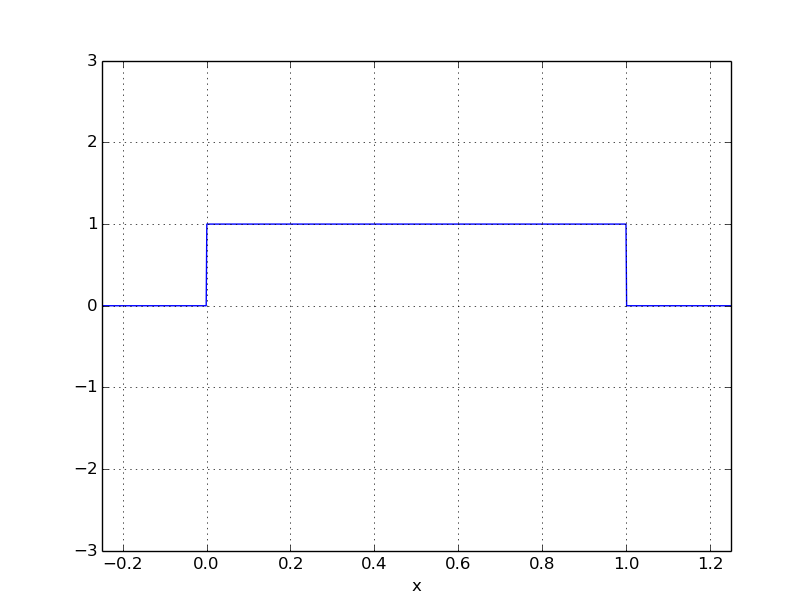
\includegraphics[width=3in]{qlmwphi0.png}
\label{fig:qlmwphi0}
}
\subfloat[Scaling Function:  $\phi^1(x)$]{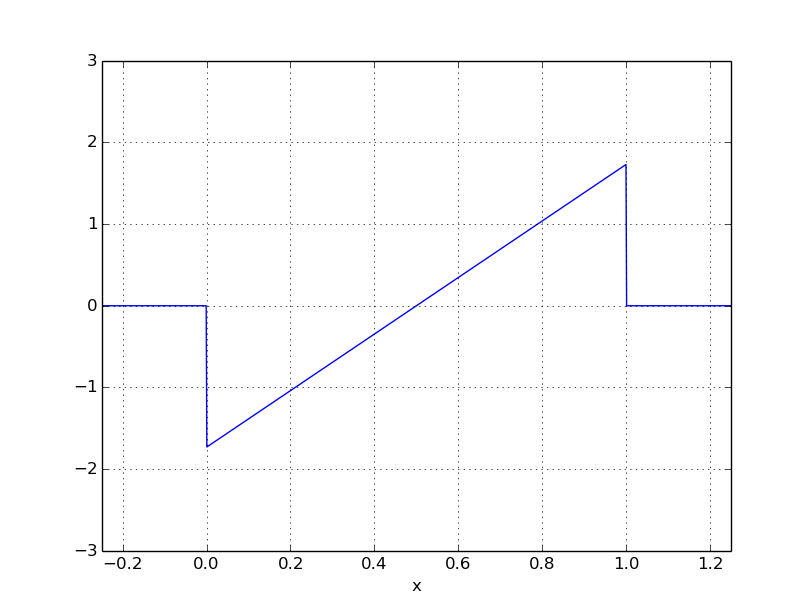
\includegraphics[width=3in]{qlmwphi1.png}
\label{fig:qlmwphi1}
}\\
\subfloat[Scaling Function:  $\phi^2(x)$]{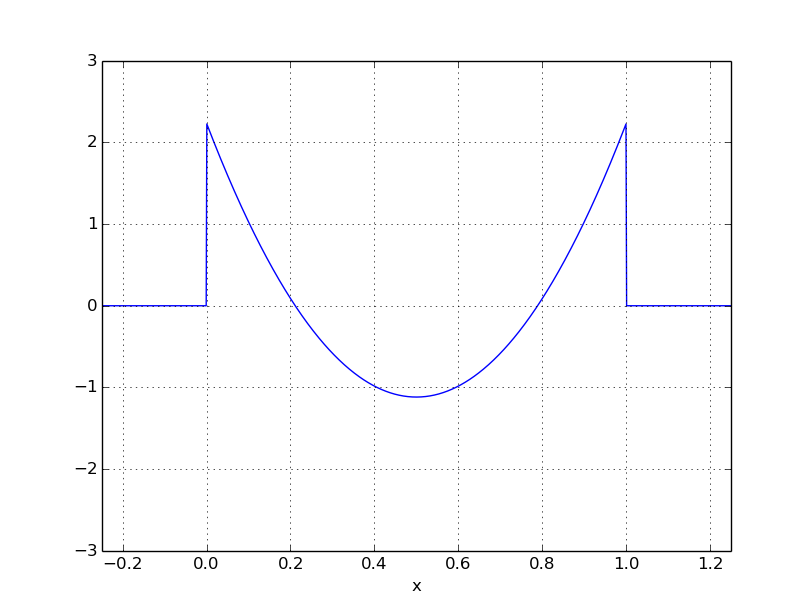
\includegraphics[width=3in]{qlmwphi2.png}
\label{fig:qlmwphi2}
}
\subfloat[Mother Wavelet Function:  $\psi^0(x)$]{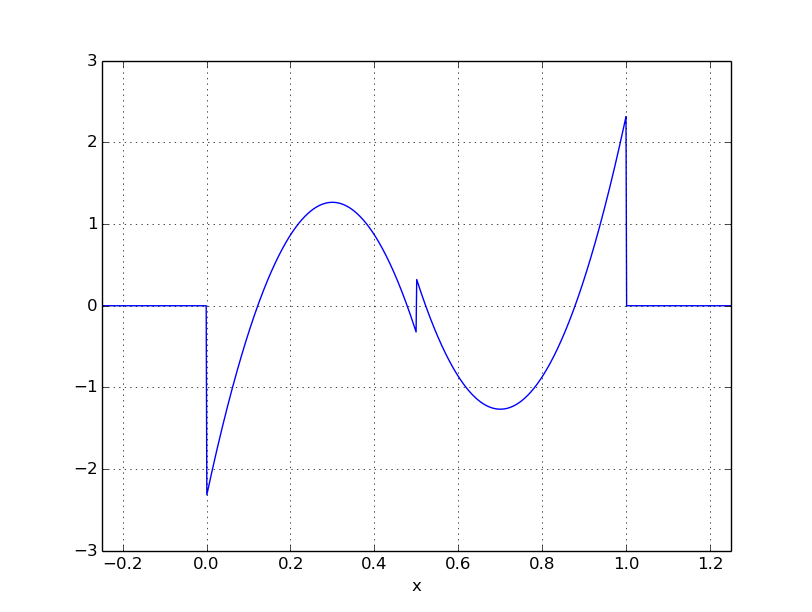
\includegraphics[width=3in]{qlmwpsi0.png}
\label{fig:qlmwpsi0}
}\\
\subfloat[Mother Wavelet Function:  $\psi^1(x)$]{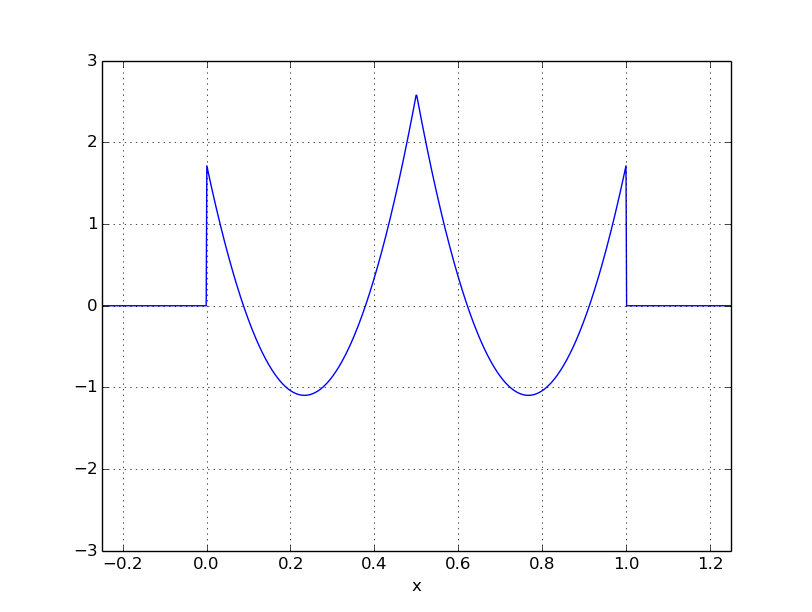
\includegraphics[width=3in]{qlmwpsi1.png}
\label{fig:qlmwpsi1}
}
\subfloat[Mother Wavelet Function:  $\psi^2(x)$]{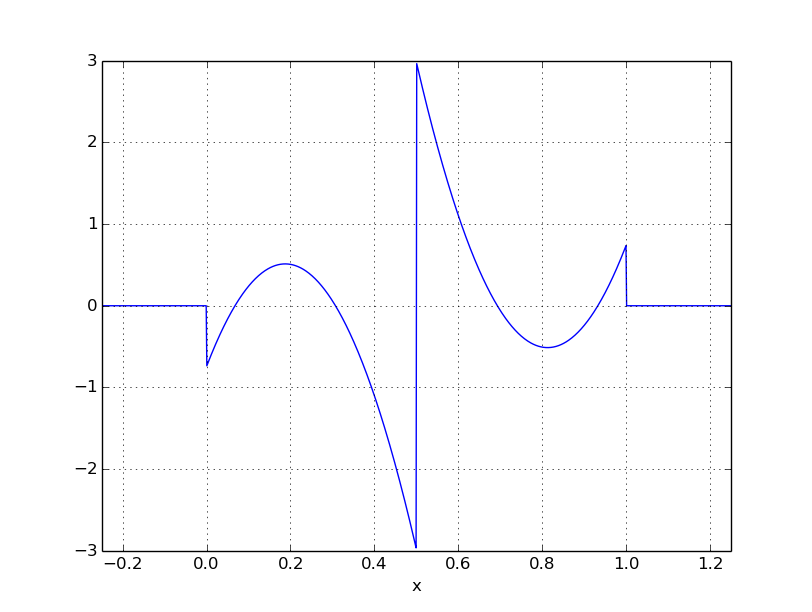
\includegraphics[width=3in]{qlmwpsi2.png}
\label{fig:qlmwpsi2}
}\\
\caption{Quadratic Legendre Multi-wavelet}
\label{fig:qlmwphipsi}
\end{figure*}



% The two scale relationship of LLMW is $4 \times 4$~matrix
% \begin{equation}
% \left[ \begin{array}{c} x_1 \\ x_2 \end{array} \right] = \begin{bmatrix} A & B \\ C & D \end{bmatrix} \times \left[ \begin{array}{c} y_1 \\ y_2 \end{array} \right]
% \end{equation}
% \underline{Find way to show this thing}



Thus QLMW basis for $L^2$ space is list of functions shown below,
\begin{equation}\label{eq:qlmwbasis}
(\phi^0_0(x),\phi^1_0(x),\phi^2_0(x),\psi^0_{n,k}(x),\psi^1_{n,k}(x),\psi^2_{n,k}(x))
\end{equation}
Where, $\quad n= 1, 2,... \quad\text{and} \quad k=0,1,2,...,2^n-1$.
If we select finite subset of the set in Equation \ref{eq:qlmwbasis}, we can form basis for space of piece-vice linear functions. For example for function space discussed in Chapter \ref{ch:projection}, we have $m=3$ and $n=4$ to get space of piece-vice constant function over standard interval of size $\frac{1}{4}$. Thus we have 4 intervals and we need 12 basis function to span this space. QLMW basis for this space is shown below
\begin{equation}\label{eq:haarbasis_n4}
(\phi^0_0(x),\phi^1_0(x),\phi^2_0(x),\psi^0_{n,k}(x),\psi^1_{n,k}(x),\psi^2_{n,k}(x))
\end{equation}
where,$\quad n=1 \quad \text{and} \quad k=0,1,2,...,2^n-1$. Use of QLMW wavelet as basis for space for approximating radiosity function is described in Chapter \ref{ch:waveletprojection}.

% To construct the linear Legendre multi-wavelets, we first define scaling
% functions φ 0 (x) and φ 1 (x) as:
% √
% φ 0 (t) = 1, φ 1 (t) = 3 (2t − 1) , 0 ≤ t < 1.
%  Multi-wavelets are class of wavelet 
% Use of LLMW and QLMW wavelet as basis for space used approximating radiosity function is described in Chapter \ref{ch:waveletprojection}.
% \underline{two scale relationship}
 
 